\section{Quadrotor simulation model}
เราได้ใช้โปรแกรม Simulink จำลองการทำงานของ quadrotor โดยจะแบ่งออกเป็นสองส่วน คือ
\vspace{-10pt}
\begin{enumerate}[label=\arabic*), leftmargin=1.5cm]
	\setlength\itemsep{-0.25em}
	\item อัตราการเปลี่ยนแปลงความเร่งเชิงเส้นโดยถูกเขียนขึ้นจากทฤษฏีที่กล่าวไปในบทที่ 2
	\item อัตราการเปลี่ยนแปลงความเร่งเชิงมุมโดยถูกเขียนขึ้นจากทฤษฏีที่กล่าวไปในบทที่ 2
\end{enumerate}
\vspace{-15pt}
\begin{figure}[!ht]
	\centering
	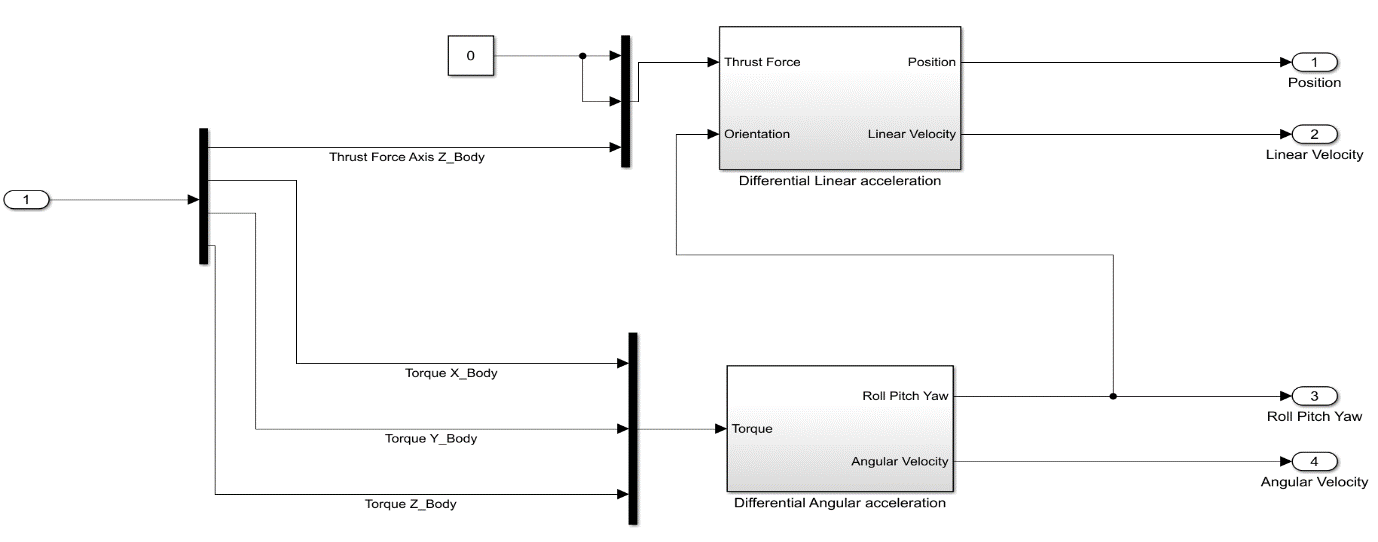
\includegraphics[width=0.8\textwidth]{images/simulink/sim_dynamic_all.png}
	\caption{แบบจำลอง quadrotor ในโปรแกรม simulink}
\end{figure}

\subsection{อัตราการเปลี่ยนแปลงความเร่งเชิงเส้น}
\begin{figure}[!ht]
	\centering
	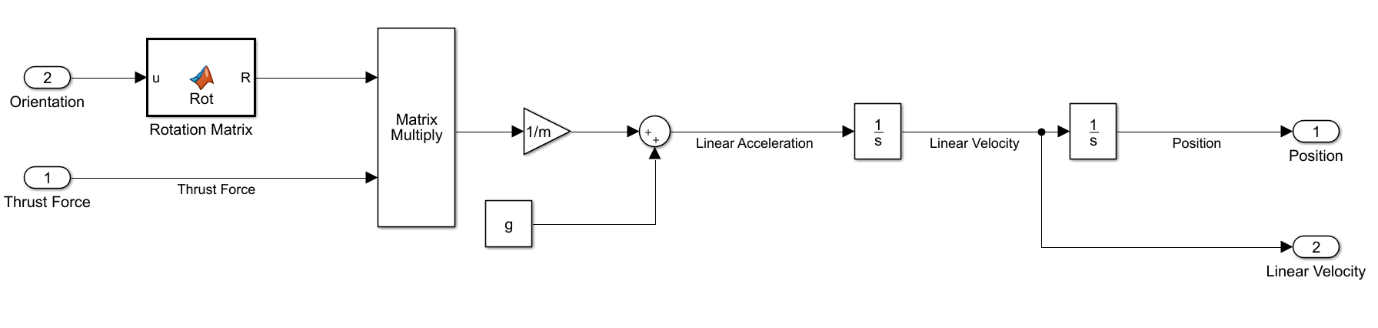
\includegraphics[width=0.95\textwidth]{images/simulink/linear_acce.png}
	\caption{อัตราการเปลี่ยนแปลงความเร่งเชิงเส้น}
\end{figure}
\vspace{-10pt}
\paragraph*{Input}
เป็นแรงขับที่กระทำกับ quadrotor และทิศทางการหมุนของ quadrotor
\paragraph*{Output}
เป็นตำแหน่งและความเร็วเชิงเส้นของ quadrotor
\vspace{15pt}
\subsection{อัตราการเปลี่ยนแปลงความเร่งเชิงมุม}
\begin{figure}[!ht]
	\centering
	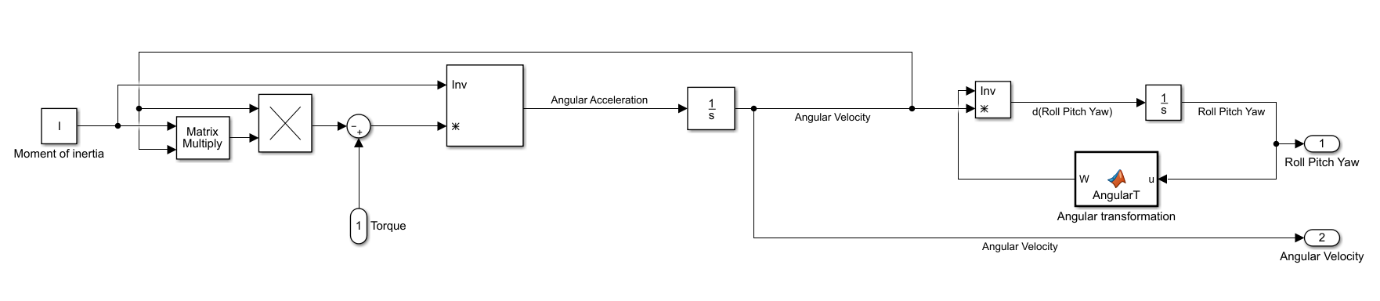
\includegraphics[width=0.95\textwidth]{images/simulink/angular_acce.png}
	\caption{อัตราการเปลี่ยนแปลงความเร่งเชิงมุม}
\end{figure}
\vspace{-10pt}
\paragraph*{Input}
เป็นแรงบิดที่กระทำกับ quadrotor
\paragraph*{Output}
เป็นทิศทางการหมุนของ quadrotor และความเร็วเชิงมุมของ quadrotor

\clearpage
\subsection{ผลการทดลอง}
กำหนดค่าเริ่มต้นต่างๆของ quadrotor ที่ใช้กับการทดลองดังนี้


\begin{center}
    \begin{tabular}{ | c | c | c | } 
    \hline
    ตัวแปร & ค่า & หน่วย \\ 
    \hline
    \hline
    $I_x$ & 0.01152 & $kgm^2$ \\ 
    \hline
    $I_y$ & 0.01152 & $kgm^2$ \\
    \hline
    $I_z$ & 0.0218 & $kgm^2$ \\
    \hline
    $g$ & 9.80665 & $m/s^2$ \\
    \hline
    $m$ & 1.477 & $kg$ \\
    \hline
    $L$ & 0.26 & $m$ \\
    \hline
    \end{tabular}
\end{center}

\subsubsection{Hover quadrotor}
ทดลอง Simulation โดยการใส่แรงขับที่กระทำให้ quadrotor สามารถลอยตัวอยู่ได้โดยไม่ร่วงลงตามแรงโน้มถ่วงของโลก

\begin{equation}
    \begin{array}{c}
    {F = ma}\\
    {F = 1.477 \times 9.80665}
    \label{equ:newton_law}
    \end{array}
\end{equation}
\begin{center}
    \begin{tabular}{ | c | c | c | } 
    \hline
    Thrust force Z & 14.48442205 & $Nm$ \\ 
    \hline
    Torque X & 0 & $Nm$ \\ 
    \hline
    Torque Y & 0 & $Nm$ \\ 
    \hline
    Torque Z & 0 & $Nm$ \\ 
    \hline
    \end{tabular}
\end{center}
\begin{figure}[!ht]
	\centering
	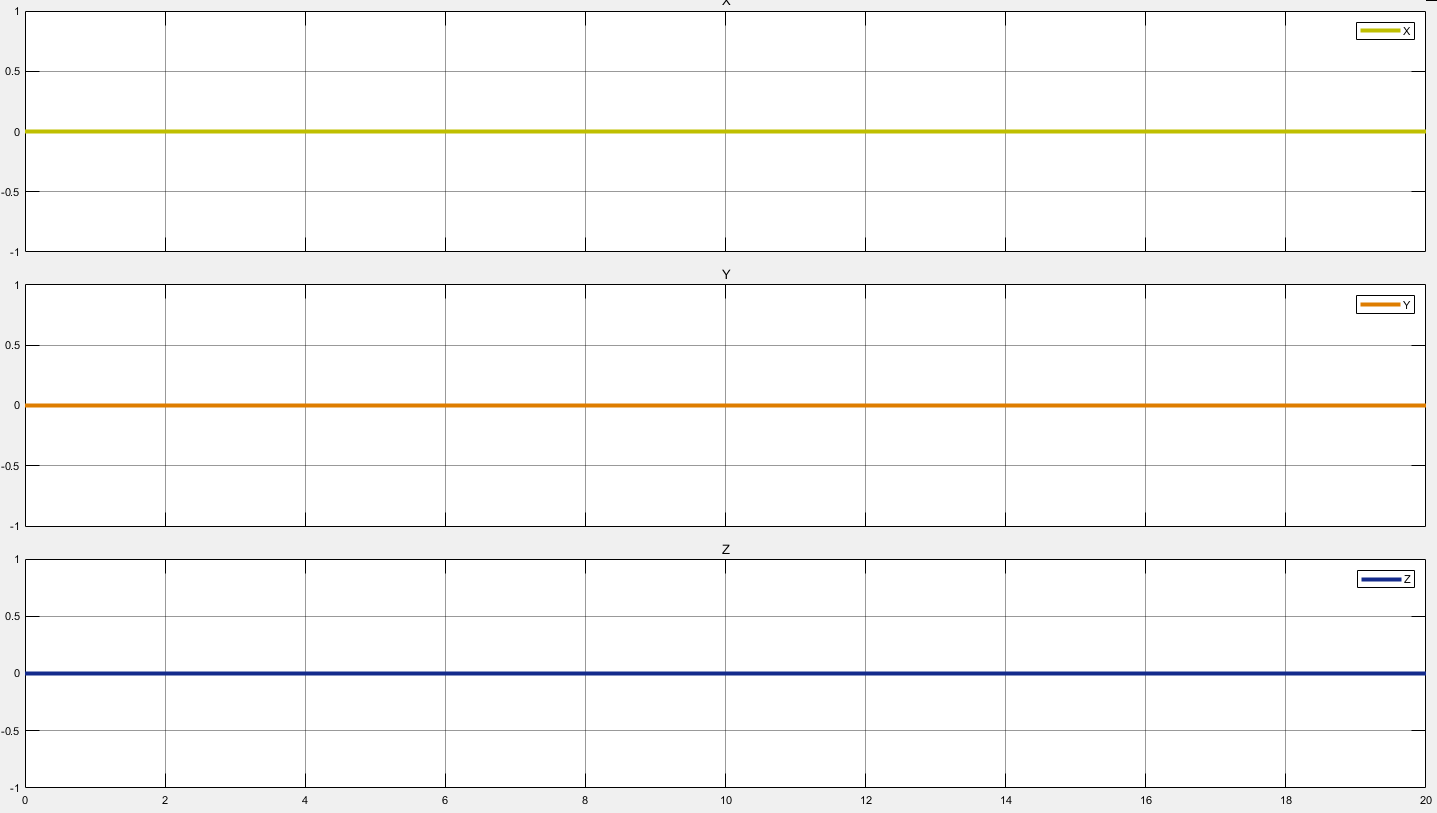
\includegraphics[width=0.95\textwidth]{images/simulink/test_hover.png}
	\caption{กราฟแสดงตำแหน่งของ quadrotor}
\end{figure}

จากผลการทดลอง quadrotor สามารถลอยอยู่ได้ที่ตำแหน่ง $x=0$, $y=0$ และ $z=0$ โดยไม่ร่วงลงมาตามแรงโน้มถ่วงของโลก

\clearpage
\subsubsection{Climb up quadrotor}
ทดลอง Simulation โดยการใส่แรงขับที่กระทำให้ quadrotor สามารถลอยตัวขึ้นไปในอากาศได้

\begin{equation}
    \begin{array}{c}
    {F > ma}\\
    {F > 1.477 \times 9.80665}
    \label{equ:newton_law}
    \end{array}
\end{equation}
\begin{center}
    \begin{tabular}{ | c | c | c | } 
    \hline
    Thrust force Z & 15.48442205 & $Nm$ \\ 
    \hline
    Torque X & 0 & $Nm$ \\ 
    \hline
    Torque Y & 0 & $Nm$ \\ 
    \hline
    Torque Z & 0 & $Nm$ \\ 
    \hline
    \end{tabular}
\end{center}
\begin{figure}[!ht]
	\centering
	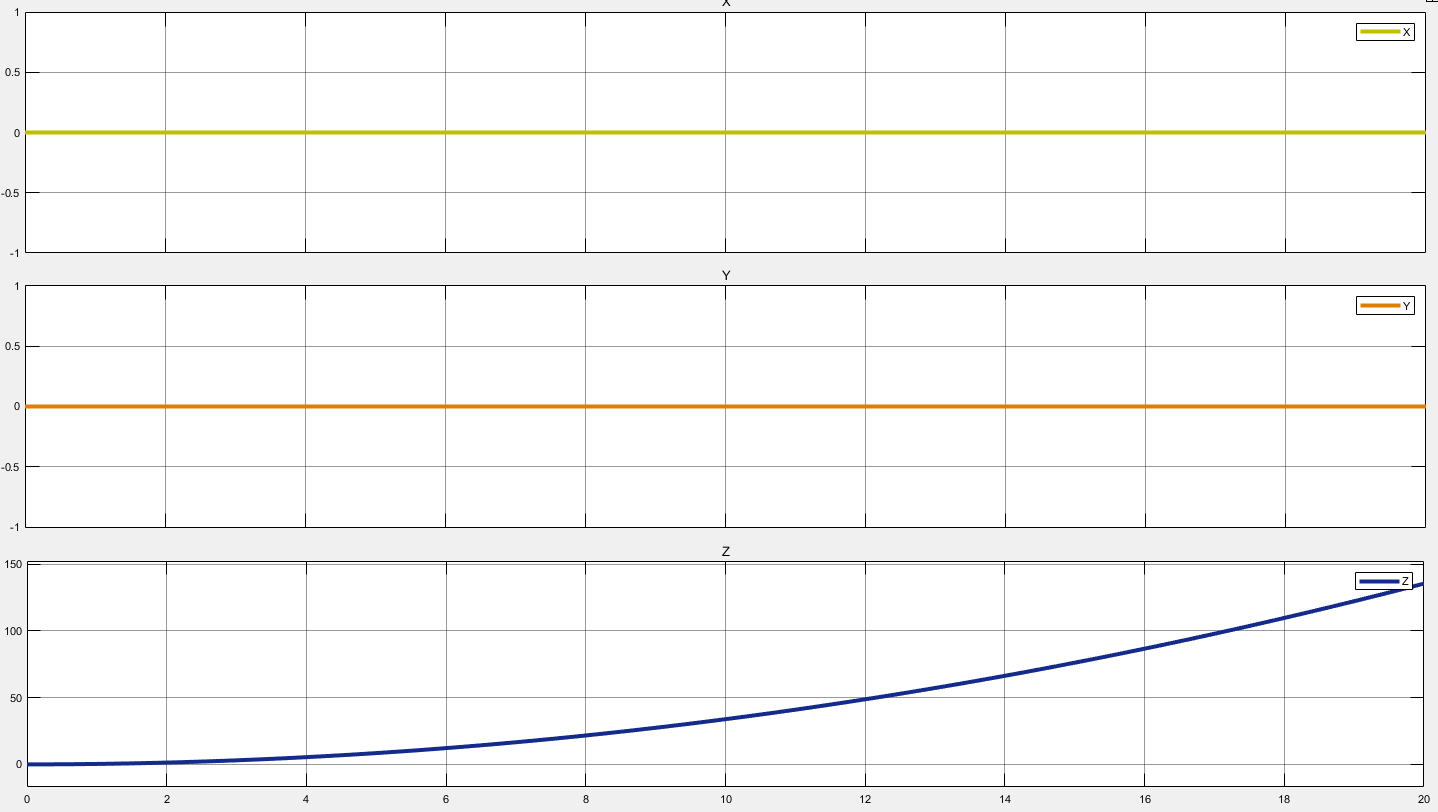
\includegraphics[width=0.95\textwidth]{images/simulink/test_climbup.png}
	\caption{กราฟแสดงตำแหน่งของ quadrotor}
\end{figure}

จากผลการทดลอง quadrotor สามารถเคลื่อนที่ลอยขึ้นไปในทิศทางตามแนวแกน Z ได้
